\section{Regression- CFRP NASA}
\label{Regression- CFRP NASA}
Composite materials, particularly Carbon Fiber Reinforced Plastics (CFRPs), have increasingly found utility in aerospace applications due to their remarkable strength-to-weight ratios. NASA has amassed significant datasets on CFRPs, making it a cornerstone in understanding and modeling the fatigue life of these materials. While traditional regression methods, such as those discussed by Sun and Verrilli~\cite{sun2002fatigue}, have provided valuable insights into the behavior of composites, the advent of deep learning techniques presents an opportunity to further refine predictive accuracy. In this study, we introduce a Convolutional Neural Network (CNN) model for predicting the S-N (Stress vs. Number of Cycles) curve, or end-of-life curve, of CFRPs using the NASA dataset. The approach seeks to leverage the nuanced, hierarchical feature extraction capabilities inherent to CNNs. Preliminary results indicate that our CNN-based regression model offers improved predictive accuracy when compared to classical regression models, especially in the presence of complex, non-linear data patterns observed in laminated composite structures. Such advancements have the potential to significantly enhance our understanding of fatigue life, damage mechanisms~\cite{talreja2012damage}, and the probabilistic nature of failures in composite materials~\cite{glaessgen2009probabilistic}. By employing CNNs for this task, we anticipate a transformative change in the way aerospace industries approach the design and safety evaluation of composite structures. One common representation of fatigue life is the S-N curve, given by:
\begin{equation}
    S = aN^b
\end{equation}
where \(S\) is the stress amplitude, \(N\) is the number of cycles leading to failure, and \(a\) and \(b\) are material constants. 

While traditional regression methods, such as those discussed by Sun and Verrilli~\cite{sun2002fatigue}, have provided valuable insights into the behavior of composites, the advent of deep learning techniques presents an opportunity to further refine predictive accuracy. 

In this study, we introduce a Convolutional Neural Network (CNN) model for predicting the S-N curve of CFRPs using the NASA dataset. The approach seeks to leverage the nuanced, hierarchical feature extraction capabilities inherent to CNNs. Preliminary results indicate that our CNN-based regression model offers improved predictive accuracy when compared to classical regression models, especially in the presence of complex, non-linear data patterns observed in laminated composite structures. Such advancements have the potential to significantly enhance our understanding of fatigue life, damage mechanisms~\cite{talreja2012damage}, and the probabilistic nature of failures in composite materials~\cite{glaessgen2009probabilistic}. By employing CNNs for this task, we anticipate a transformative change in the way aerospace industries approach the design and safety evaluation of composite structures.

\subsection{Initialization and Data Loading}

\begin{lstlisting}
% Start a parallel pool
if isempty(gcp('nocreate'))
    parpool;
end

% Initialize tables for Layup 1, Layup 2, and Layup 3
initTable = table('Size', [0, 14], 'VariableTypes',..
repmat({'double'}, 1, 14), ...
... % Additional initialization code omitted for brevity
\end{lstlisting}

The code initiates by ensuring that a parallel computing pool is started, likely to facilitate parallelized operations in later stages. It then establishes three empty tables for different configurations of the composite material and defines an array, `dirr`, with directories of `.mat` files that presumably store test data. 
\subsection{Data Extraction and Processing}

The data extraction process is built on iterative loops that navigate through directories and their respective `.mat` files, extracting crucial pieces of data. Here's a brief breakdown:

\begin{enumerate}
    \item \textbf{Directory Looping}: The code initializes with a list of directories ($\texttt{dirr}$). It loops through each one, aiming to process every `.mat` file inside them.
    
    \begin{lstlisting}
for d = 1:length(dirr)
    matFiles = dir(dirr{d});
    ...
\end{lstlisting}
    
    \item \textbf{Loading Files}: For each directory, it lists all the `.mat` files and loops through them, loading them sequentially.
    
    \begin{lstlisting}
for i = 1:length(matFiles)
    filePath = fullfile(matFiles(i).folder, matFiles(i).name);
    tempData = load(filePath);
    ...
\end{lstlisting}

    \item \textbf{Data Extraction}: If the loaded file has a $\texttt{coupon}$ field, it starts the extraction. Direct fields like $\texttt{load}$ and $\texttt{cycles}$ are fetched immediately. When $\texttt{path\_data}$ is present, additional attributes related to actuator and sensor are extracted. Certain features, such as mean and energy, are computed directly in this step.
    
    \begin{lstlisting}
if isfield(tempData, 'coupon')
    ...
    if isfield(tempData.coupon, 'path_data')
        ...
\end{lstlisting}

    \item \textbf{Row Creation and Appending}: After extraction, a new data row is constructed and appended to one of the initialized tables, depending on the directory of origin.
    
    \begin{lstlisting}
newRow = table(...);
if contains(dirr{d}, 'Layup1')
    layup1Table = [layup1Table; newRow];
...
\end{lstlisting}

    \item \textbf{Reiteration}: This entire process is reiterated until all `.mat` files across all directories are processed.
\end{enumerate}

This iterative data extraction method ensures that all critical information from the `.mat` files is processed and neatly organized into the respective tables for each layup type.

\subsection{Data Cleaning and Saving}

\begin{lstlisting}
function cleanedTable = removeEmptyRows(inputTable)
... % Function implementation omitted for brevity
\end{lstlisting}

Upon completion of data loading, the `removeEmptyRows` function cleans each layup table by removing rows with empty or `NaN` values. This is a standard step in data preprocessing. Finally, the cleaned layup tables are saved as `.mat` files.

\subsection{Data Loading and Preparation}

The first part of the code is about loading the required data and preparing it for analysis:

\begin{lstlisting}
load('layup1Table.mat')
...
dataArray = table2array(layup1Table);
...
\end{lstlisting}

Here, the data is loaded from the \texttt{layup1Table.mat} file and then converted to an array for further processing\cite{datapreprocess}.

\subsubsection{Training and Test Set Partition}

Data is partitioned into training and test sets. 70\% of the data is used for training, and 30\% for testing. 

\begin{lstlisting}
n = size(featureMatrix, 1);
...
XTrain = cell2mat(featureMatrix(shuffleIdx(1:nTrain), :));
...
\end{lstlisting}

The dataset is also shuffled to ensure randomness\cite{datapreprocess}.

\subsubsection{Data Normalization}

Data normalization is an essential step before training neural networks:

\begin{lstlisting}
XTrain_norm = (XTrain - featureMin) ./ (featureMax - featureMin);
...
\end{lstlisting}

This step scales the data between 0 and 1, ensuring all features have the same scale\cite{neuralnet}.

\subsection{Neural Network Design}

The neural network is designed for regression analysis, which is evident from the subsequent evaluation of its predictions against continuous output values.

\subsubsection{Neural Network Architecture}
\begin{enumerate}
    \item \textbf{Hidden Layer Configuration}: The neural network has one hidden layer. The number of neurons in this hidden layer is defined by \texttt{hiddenLayerSize}, which is set to 10 in the code.

    \begin{lstlisting}[language=Matlab]
    hiddenLayerSize = 10;
    \end{lstlisting}

    \item \textbf{Training Algorithm}: The Levenberg-Marquardt backpropagation algorithm, represented by \texttt{trainlm}, is used for training. It's known for its efficiency and speed, especially for small and medium-sized datasets.

    \begin{lstlisting}[language=Matlab]
    trainFcn = 'trainlm';
    \end{lstlisting}

    \item \textbf{Network Creation}: The \texttt{fitnet} function is utilized to create a feedforward backpropagation network. This function initializes the weights and biases of the network.

    \begin{lstlisting}[language=Matlab]
    net = fitnet(hiddenLayerSize, trainFcn);
    \end{lstlisting}
\end{enumerate}

\subsubsection{Training Configuration}
\begin{enumerate}
    \item \textbf{Epochs}: The maximum number of epochs (iterations) the network should train for is set to 100. An epoch is one forward and backward pass of all the training examples.

    \begin{lstlisting}[language=Matlab]
    net.trainParam.epochs = 100;
    \end{lstlisting}

    \item \textbf{Learning Rate}: The rate at which the network updates its weights and biases. A rate of 0.05 is specified, meaning the network makes relatively small adjustments to the weights and biases during training.

    \begin{lstlisting}[language=Matlab]
    net.trainParam.lr = 0.05;
    \end{lstlisting}

    \item \textbf{Performance Goal}: The training will stop if the mean squared error falls below \texttt{1e-5}.

    \begin{lstlisting}[language=Matlab]
    net.trainParam.goal = 1e-5;
    \end{lstlisting}
    
    \item \textbf{Other Parameters}: There are other configuration settings related to performance gradient, display settings, and the maximum training time.
\end{enumerate}

\subsubsection{Data Division for Training, Validation, and Testing}

The dataset is divided into three parts: training, validation, and testing. Specifically, 70\% of the data is used for training, 15\% for validation, and 15\% for testing. Validation data assists in preventing overfitting during training.

\begin{lstlisting}[language=Matlab]
net.divideParam.trainRatio = trainFraction;
net.divideParam.valRatio = valFraction;
net.divideParam.testRatio = testFraction;
\end{lstlisting}

The neural network is then trained using the \texttt{train} function, which uses the configuration defined earlier and adjusts the network weights based on the training data.


% Layup 1 Curves
\begin{figure}[h]
    \centering
    \begin{minipage}{0.45\textwidth}
        \centering
        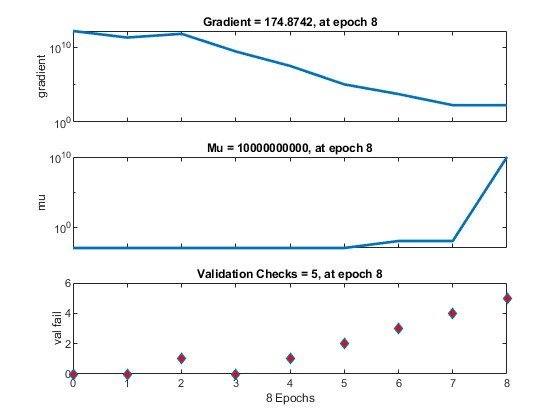
\includegraphics[width=\linewidth]{train_1.jpg}
        \caption{training state for Layup 1.}
    \end{minipage}
    \hfill
    \begin{minipage}{0.45\textwidth}
        \centering
        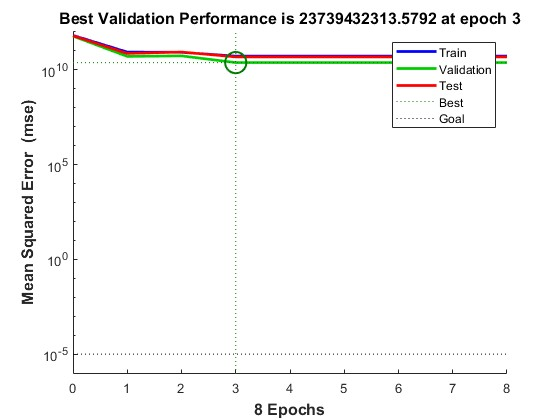
\includegraphics[width=\linewidth]{train_11.jpg}
        \caption{validation progress for Layup 1.}
    \end{minipage}
\end{figure}

% Layup 2 Curves
\begin{figure}[h]
    \centering
    \begin{minipage}{0.45\textwidth}
        \centering
        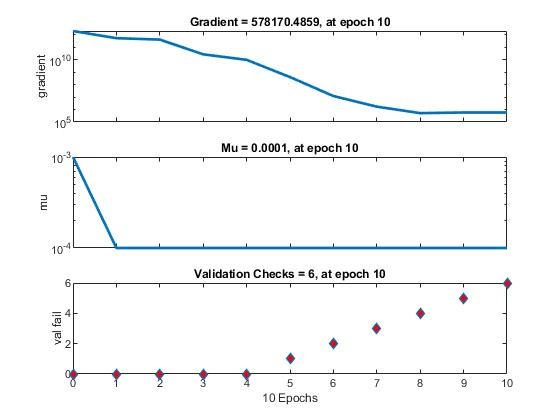
\includegraphics[width=\linewidth]{train_2.jpg}
        \caption{training state for Layup 2.}
    \end{minipage}
    \hfill
    \begin{minipage}{0.45\textwidth}
        \centering
        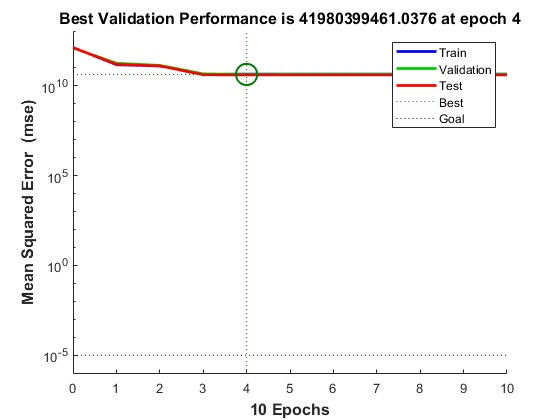
\includegraphics[width=\linewidth]{train_22.jpg}
        \caption{validation progressr Layup 2.}
    \end{minipage}
\end{figure}

% Layup 3 Curves
\begin{figure}[h]
    \centering
    \begin{minipage}{0.45\textwidth}
        \centering
        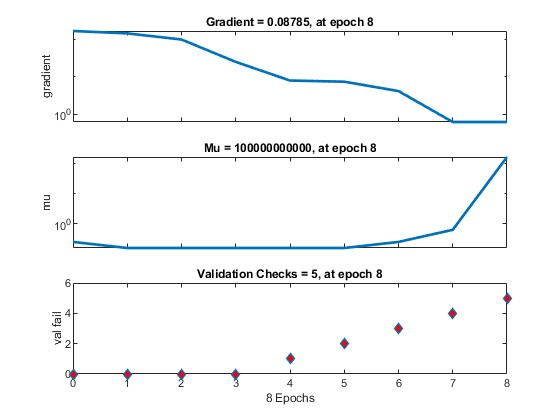
\includegraphics[width=\linewidth]{train_3.jpg}
        \caption{training state for Layup 3.}
    \end{minipage}
    \hfill
    \begin{minipage}{0.45\textwidth}
        \centering
        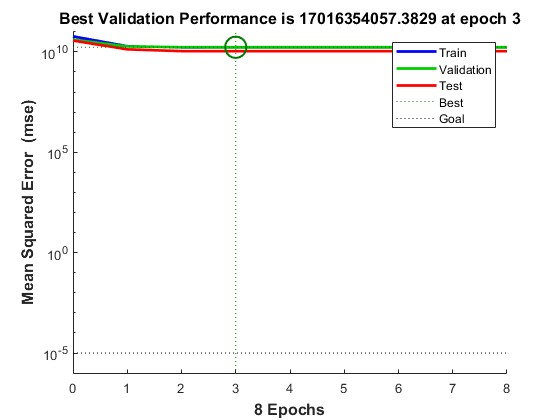
\includegraphics[width=\linewidth]{train_33.jpg}
        \caption{validation progress for Layup 3.}
    \end{minipage}
\end{figure}
By understanding this design, one can make informed decisions about potential modifications or optimizations depending on the specific requirements of the application or the nature of the dataset.
\subsection{Model Evaluation: \texttt{evaluateNNModel} Function}

The function \texttt{evaluateNNModel} serves as an all-encompassing method for training and evaluating a neural network. In this section, we'll dissect its operation.

\subsubsection{Function Inputs and Outputs}

\begin{itemize}
    \item \textbf{Inputs}:
    \begin{itemize}
        \item \texttt{net}: The untrained neural network architecture.
        \item \texttt{XTrain\_norm}: Normalized feature matrix of the training set.
        \item \texttt{YTrain\_norm}: Normalized label/output matrix of the training set.
        \item \texttt{XTest\_norm}: Normalized feature matrix of the test set.
        \item \texttt{YTest\_norm}: Normalized label/output matrix of the test set.
        \item \texttt{threshold}: User-defined value for detecting overfitting.
    \end{itemize}
    \item \textbf{Outputs}:
    \begin{itemize}
        \item \texttt{mseTrain}: MSE on the training set.
        \item \texttt{mseTest}: MSE on the test set.
        \item \texttt{isOverfitting}: A boolean indicating potential overfitting.
    \end{itemize}
\end{itemize}

\subsubsection{Function Operation}

\begin{enumerate}
    \item \textbf{Training the Neural Network}:
    
    The neural network is trained using the normalized training data.
    \begin{lstlisting}
[net, tr] = train(net, XTrain_norm', YTrain_norm');
    \end{lstlisting}
    
    \item \textbf{Prediction on Training and Test Sets}:
    
    Predictions are fetched from the trained network.
    \begin{lstlisting}
yPredTrain = net(XTrain_norm');
yPredTest = net(XTest_norm');
    \end{lstlisting}
    
    \item \textbf{Calculating MSE for Training and Test Sets}:
    
    MSE is calculated for both the training and test sets.
    \begin{lstlisting}
mseTrain = mean((yPredTrain' - YTrain_norm).^2);
mseTest = mean((yPredTest' - YTest_norm).^2);
    \end{lstlisting}
    
    \item \textbf{Displaying the MSE Values}:
    
    The calculated MSE values are printed out.
    \begin{lstlisting}
fprintf('MSE on Training Set: \%f\n', mseTrain);
fprintf('MSE on Test Set: \%f\n', mseTest);
    \end{lstlisting}
    
    \item \textbf{Checking for Overfitting}:
    
    The function checks if the model might be overfitting, based on the comparison of MSE values.
    \begin{lstlisting}
isOverfitting = false;
if mseTrain < mseTest
    difference = mseTest - mseTrain;
    if difference > threshold
        disp('Warning: The model might be overfitting.');
        isOverfitting = true;
    end
else
    disp('The model seems to generalize well.');
end
    \end{lstlisting}
\end{enumerate}

In essence, \texttt{evaluateNNModel} facilitates the training, prediction, and evaluation of a neural network's performance, particularly emphasizing the detection of overfitting through the MSE values comparison.

\subsection{Curve Fitting}

Curve fitting is used in the latter parts of the code:

\begin{lstlisting}
[fitresult, gof] = fit( xData, yData, ft, opts );
...
\end{lstlisting}

This step tries to establish a relationship between predicted cycles and other parameters, possibly trying to understand fatigue life or other similar relationships\cite{curvefit}.

\subsection{Conclusion}

In the following section, we present a comparison of the results obtained from the analysis of three different layups. The metrics under consideration include the Mean Squared Error (MSE) for both training and test datasets, as well as the correlation coefficient (\( R \) value). Additionally, visual representations in the form of the predicted S-N curve and the RUL curve for each layup are provided.
as it can deduced from Table 2.1, the MSE value for the train data sets is greater than that for the value for the train, proving that the data trained network is not over fitted.


\begin{table}[h]
    \centering
    \begin{tabularx}{\textwidth}{|c|X|X|X|}
        \hline
        Layup & MSE (Train) & MSE (Test) & \( R \) Value \\
        \hline
        Layup 1 & 0.075019 \&\0.064859  & 0.072509 \&\0.059717 & 0.74152 \\
        Layup 2 & 0.071039 \&\0.066820 & 0.058086\&\0.053494 & 0.66806 \\
        Layup 3 & 0.071793\&\0.060680 & 0.067616 \&\0.051012  & 0.65694 \\
        \hline
    \end{tabularx}
    \caption{Comparison of MSE values and \( R \) values for the three layups.}
\end{table}

% Layup 1 Curves
\begin{figure}[h]
    \centering
    \begin{minipage}{0.45\textwidth}
        \centering
        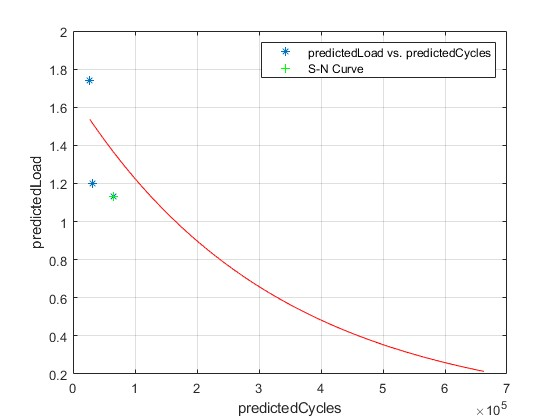
\includegraphics[width=\linewidth]{s_n_1.jpg}
        \caption{Predicted S-N Curve for Layup 1.}
    \end{minipage}
    \hfill
    \begin{minipage}{0.45\textwidth}
        \centering
        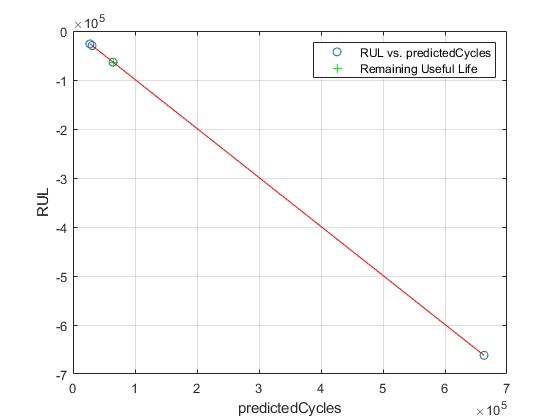
\includegraphics[width=\linewidth]{rul_1.jpg}
        \caption{RUL Curve for Layup 1.}
    \end{minipage}
\end{figure}

% Layup 2 Curves
\begin{figure}[h]
    \centering
    \begin{minipage}{0.45\textwidth}
        \centering
        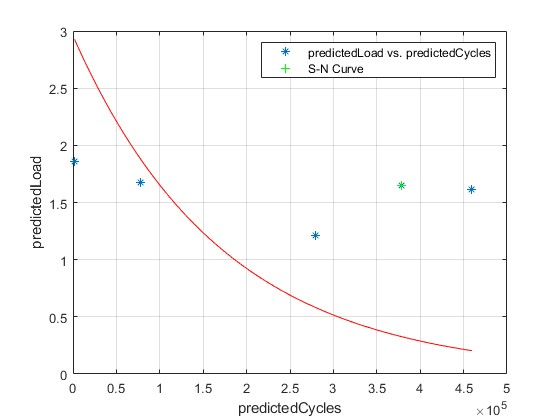
\includegraphics[width=\linewidth]{s_n_2.jpg}
        \caption{Predicted S-N Curve for Layup 2.}
    \end{minipage}
    \hfill
    \begin{minipage}{0.45\textwidth}
        \centering
        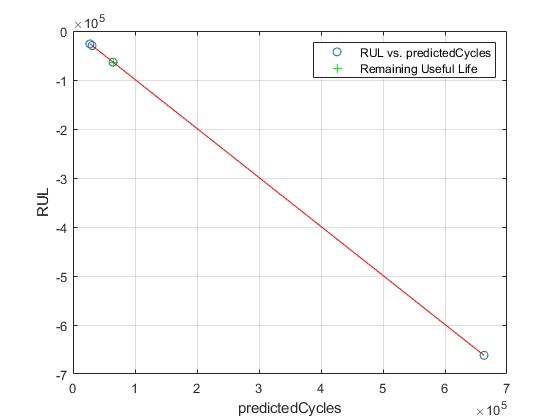
\includegraphics[width=\linewidth]{rul_1.jpg}
        \caption{RUL Curve for Layup 2.}
    \end{minipage}
\end{figure}

% Layup 3 Curves
\begin{figure}[h]
    \centering
    \begin{minipage}{0.45\textwidth}
        \centering
        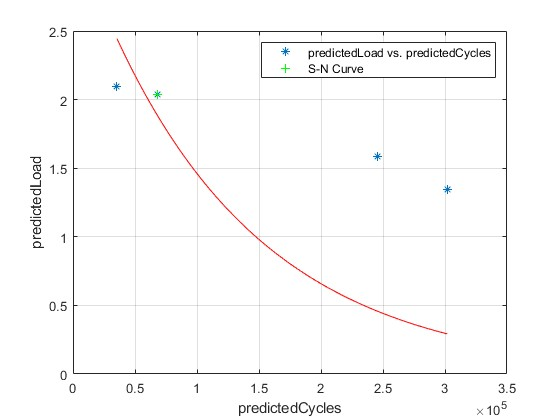
\includegraphics[width=\linewidth]{s_n_3.jpg}
        \caption{Predicted S-N Curve for Layup 3.}
    \end{minipage}
    \hfill
    \begin{minipage}{0.45\textwidth}
        \centering
        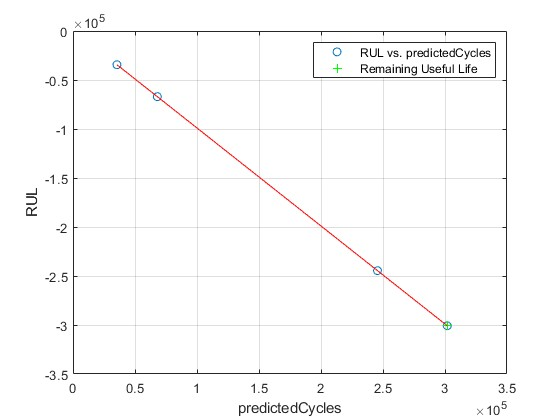
\includegraphics[width=\linewidth]{rul_3.jpg}
        \caption{RUL Curve for Layup 3.}
    \end{minipage}
\end{figure}





